\graphicspath{{../images/}}
\section{Проблема шумоподавления}
При шумоподавлении особенную роль играет его природа. Почему он возник, зависит ли шум от изображения, является он аддитивным
или мультипликативным, а так же модель шума. 

Источники шума\cite{Gonzalez}:
\begin{itemize}
	\item неидеальное оборудование для захвата изображения — видеокамера, сканер и
	т.п.;
	\item плохие условия съемки — например, сильные шумы, возникающие при
	ночной фото/видеосъемке;
	\item помехи при передаче по аналоговым каналам — наводки от источников
	электромагнитных полей, собственные шумы активных компонентов
	(усилителей) линии передачи
\end{itemize}

Типы шума
\begin{itemize}
	\item Аддитивный шум
	\item Мультипликативный шум
\end{itemize}

Кроме всего прочего, так же различают и модели шума.
\begin{itemize}
	\item Гауссовский шум
	\item Белый шум
	\item Импульсный шум
	\item Спекл-шум
	\item Паусоновский шум
\end{itemize}

В подавляющем числе случаев шум на цифровых изображениях является аддитивным гауссовым. Так
как именно он зачастую появляется при формировании изображения. Он характеризуется добавленем какого-то
значения из нормального распределения с конечным среднеквадратичным отклонениме. Наложение шума
на изображение можно описать следующим образом.
\begin{equation}\label{eModelNoise}
	y(i,j)=x(i,j)+n(i,j)
\end{equation}
где
\begin{itemize}
	\item y - защумленное изображение
	\item x - оригинальное изображеие
	\item n - шум имеющий распределение гаусса
	\item i,j - координаты пикселя
\end{itemize}

В свою очередь распределение гаусса можно задать формулой приведенной ниже.

\begin{equation}\label{eGaussNoise}
	G(x)=\frac{N}{\sqrt{2\pi}\sigma}exp(-\frac{(x-\mu)^2}{\sigma^2})	
\end{equation}
\begin{itemize}
	\item $\sigma$ - дисперсия 
	\item $\mu$ - среднеквадратичное отклонение
\end{itemize}

Задачей шумоподавления является нахождения такого изображения $x'$, которое было бы максимально похоже на оригинальное изображение $x$. 
%%неверно, удалить. Найти определение линейных фильтров.
Наиболее простыми методами являются, так называемые, линейные или локальные фильтры. Они основаны на следующей идеи, пиксели в некоторой окрестности с наибольшей вероятности имееют приблизительно одинаковые значения. К ним относятся алгоритмы, которые берут информацию о новом значение из пикселей в некоторой окресностности: Box фильтра, фильтр гаусса и медианный фильтр. Данные фильтры не применяются на практике, так как после филтрации изображения значительно теряется и теряется информация о краях.

\subsection{Классификация фильтров}
В данной ВКР исследуются алгоритмы отнесенные к следующим классам методов шумоподавления:
\begin{itemize}
	\item Нелокальные: Bilateral, Guided, Non-Local Means.
	\item Вейвлет-преобразования: BM3D.
	\item На основе апостиорной вероятности: Markov Random Field.
	\item На основе вариаций функции: Total variation.
\end{itemize}

\subsection{Dataset}
Для исследования былы подобранны изображения различных типов, для определения, к какми классам изображения
какие фильтры применять изображения. Имеются: фотографии архитектуры, текстуры, изображения с низкой освещенностью, портреты людей, а так же комбинация некоторых. Все изображения взяты с сайта https://pixabay.com/images/search/people/. Ниже приведены экземпляры изображений.
Изображение архитектуры:
\begin{figure}[h]
\center{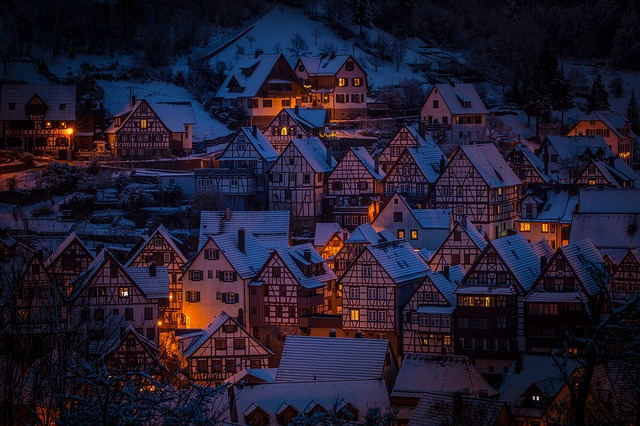
\includegraphics[width=0.4\textheight, keepaspectratio]{architecture-3076685_640.jpg}}
\caption{изображение типа архитектура}
\label{fig:Architecture}
\end{figure}
\begin{figure}[h]
	\center{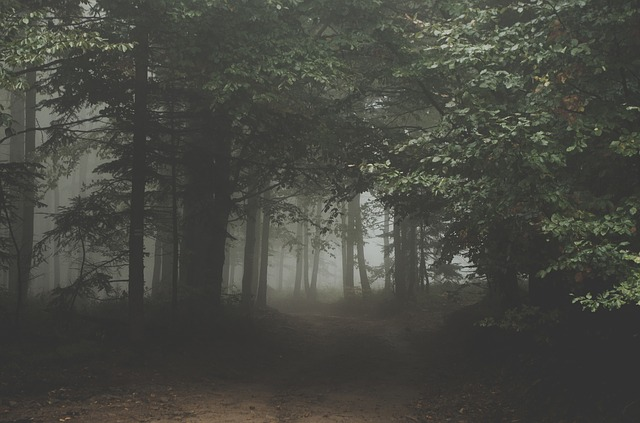
\includegraphics[width=0.4\textheight, keepaspectratio]{forest-1031022_640.jpg}}
	\caption{изображение типа плохое освещение}
	\label{fig:Night}
\end{figure}
\begin{figure}[h]
	\center{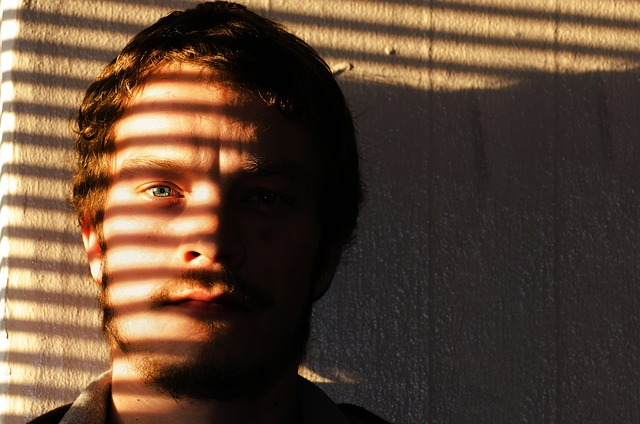
\includegraphics[width=0.4\textheight, keepaspectratio]{man-164962_640.jpg}}
	\caption{изображение типа портерт}
	\label{fig:Man}
\end{figure}
\begin{figure}[h]
	\center{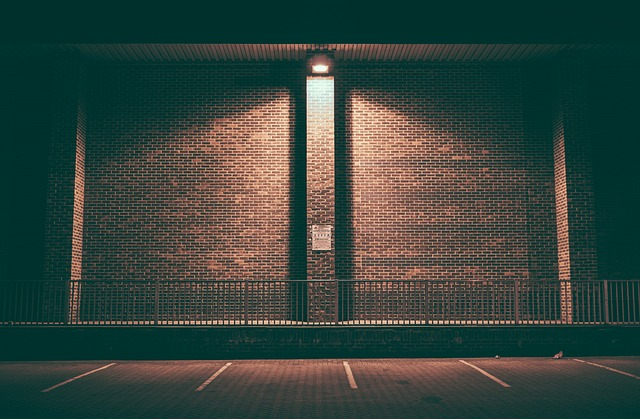
\includegraphics[width=0.4\textheight, keepaspectratio]{brick-wall-1834446_640.jpg}}
	\caption{изображение типа текстура}
	\label{fig:Texture}
\end{figure}
\begin{figure}[h]
	\center{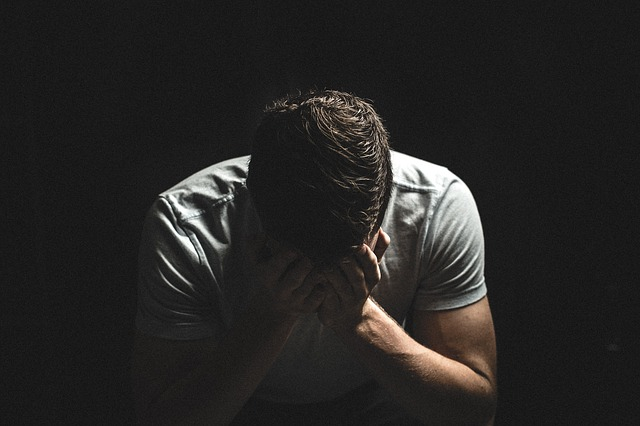
\includegraphics[width=0.4\textheight, keepaspectratio]{guy-2617866_640.jpg}}
	\caption{изображение типа текстура}
	\label{fig:Guy}
\end{figure}